\newif\ifloesung
\loesungfalse

\newif\ifenglisch
\englischtrue


\documentclass[a4paper,12pt,ngerman]{article}
\usepackage[utf8]{inputenc}
\usepackage[T1]{fontenc}     % Um die Zeichen korrekt zu kodieren
\usepackage[ngerman]{babel}
\usepackage{amssymb}  % für \Box
\usepackage{fancyhdr}
\usepackage{setspace}
\usepackage{framed}
%\usepackage{xcolor}
\usepackage{hhline}
\usepackage{longtable}
\usepackage{array}     % für m{} etc. in Tabellen
%\usepackage{booktabs}  % für \addlinespace[2ex] in Tabellen
\usepackage{graphicx}
\usepackage[export]{adjustbox}
\usepackage{caption}
\usepackage{subcaption}
%\usepackage{hyperref}  % für \autoref{...}
\usepackage{lastpage}  % für thelastepage im Header
\usepackage{paralist}  % compactenum in Unteraufgaben
\usepackage{enumitem}  % Anpassbare Enumerates/Itemizes
%\usepackage{pstricks}  % Tex-Graphiken exportiert von Dia
\usepackage{tikz}    
\usepackage{xparse}    % für neue Befehle mit variabler Anzahl von Parametern (hier \lsg)
\usepackage{soul}      % zum "verstecken" von Lösungstext
%\usepackage[plainpages=false, pdfpagelabels,colorlinks=true, pdfstartview=FitV, linkcolor=blue, citecolor=blue, urlcolor=blue]{hyperref}
\usepackage{listings}
\usepackage{eurosym}   % für das Euro-Symbol
\usepackage{verbatim}
%\usetikzlibrary{positioning,shapes,shadows,arrows.meta,calc}
\usepackage{lipsum}
\usepackage[most]{tcolorbox}

% % % % % % % % % % % % % % % % % % % % % % % % % % % % %
% Befehle zum Ein- und Ausblenden von Lösungen
%

\ifloesung
	\NewDocumentCommand\lsg{+m +g}{%
		\textcolor{red}{#1}
	}
	\newcommand{\nlsg}[1]{}
\else
	\NewDocumentCommand\lsg{+m +g}{%
		\IfNoValueF{#2}
			{#2}
			{}
	}
	\newcommand{\nlsg}[1]{#1}
\fi

% Jedes Zeichen innerhalb von \geheim{...} entfernen
% wenn die Zeichen durch etwas anderes (z.B. ?) ersetzt
% werden sollen dann \phantom{\the\SOUL@token} ersetzen 
% (z.B. durch ?)
% benötigt \usepackage{soul}
\makeatletter
\DeclareRobustCommand{\geheim}{%
  \SOUL@setup
  \def\SOUL@everytoken{%
    \phantom{\the\SOUL@token}}\SOUL@}
\makeatother

% % % % % % % % % % % % % % % % % % % % % % % % % % % % %

% % % % % % % % % % % % % % % % % % % % % % % % % % % % %
% Konfiguration der Codeausgabe mit listings
%
%\usepackage{pxfonts}  % erlaube \ttfamily in bold, geht derzeit nicht in meinem MikTex unter Windows  
\renewcommand{\ttdefault}{pcr} % Courier font auswählen, der bold erlaubt, (Alternative zu pxfonts)
\lstset{basicstyle=\ttfamily}
%\lstset{keywordstyle=\bfseries} % ist Default
% \bf hinzufügen, wenn es bold sein soll
% gilt auch für Code im Text
\lstset{keywordstyle=\bfseries}
%\lstset{keywordstyle=\bfseries\ttfamily\underbar}
%\lstset{keywordstyle=\color{blue}\ttfamily}
\lstset{stringstyle=\it}
%\lstset{stringstyle=\color{red}\ttfamily}
%\lstset{commentstyle=\ttfamily\itstyle}
%\lstset{commentstyle=\color{green}\ttfamily}
\lstset{tabsize=4}
\lstset{showtabs=false}
\lstset{language=C++}
\lstset{morekeywords={ostringstream, istringstream, stringstream, ostream}}
%\lstset{showspaces=false, 
%        showtabs=false, tab= , 
%		 keywordstyle=\blue\bfseries, 
%		 commentstyle=\it\color{greenf},%
%        showstringspaces=false, framexleftmargin=5mm, 
%		 frame=none, numbers=none, numberstyle=\tiny, 
%		 stepnumber=1, numbersep=5pt,%
%        texcl=true,escapechar=!
%}
% automatischen Zeilenumbruch erlauben  \lstset{breaklines=true}  
% automatischer Zeilenumbruch nur bei Whitespace              
\lstset{breakatwhitespace=false}
\lstset{showstringspaces=false,
        commentstyle=\color{black} 
%        morecomment=[l]{//}
}
% Coder der Lösung in rot oder ausgeblendet
\ifloesung
\lstset{morecomment=[l][\color{red}]{//=},
		morecomment=[s][\color{red}]{//+}{//-},
		morecomment=[s][\color{red}]{//l\{}{//l\}},		
		morecomment=[s][\color{red}]{/*l\{*/}{/*l\}*/}
}
\else
% mit [is] wird der Kommentar ignoriert und nicht ausgegeben ==> Platz für Lösung einplanen
% [il] funktioniert nicht, löscht alles Folgende
\lstset{morecomment=[is]{//=}{.},
	 	morecomment=[is]{//+}{//-},
		morecomment=[is]{//l\{}{//l\}},	 	
	 	morecomment=[is]{/*l\{*/}{/*l\}*/}
}
\fi
% Umlaute in Listings zu erlauben
\lstset{literate=      
{Ö}{{\"O}}1       
{Ä}{{\"A}}1
{Ü}{{\"U}}1
{ß}{{\ss}}2
{ü}{{\"u}}1
{ä}{{\"a}}1
{ö}{{\"o}}1
{~}{$\sim$}{1}     % hochgestellte Tilde in eine in Mitte
                   % gestellte Tilde umwandeln
}
% Programmcode im Text
\newcommand\pct[1]{\lstinline!#1!}

% % % % % % % % % % % % % % % % % % % % % % % % % % % %

% % % % % % % % % % % % % % % % % % % % % % % % % % % %
% Konfiguration für tikz
%

%\definecolorset{rgb}{}{}%
%{lightyellow,1,1,0.6;%
% lightblue,0.529,0.81,1;%
% lightred,1,0.6,0.6;%
% greenf,0,0.5647,0%
%}

%\pgfrealjobname{pruefung}
%\usetikzlibrary{shapes,arrows,intersections,backgrounds}
%\usetikzlibrary{decorations.markings, decorations.pathmorphing,patterns,snakes}
%\usetikzlibrary{circuits.ee.IEC, circuits.logic.IEC}
%tikzstyle{ST2style} = [auto, line width=1pt, >=stealth]

%\tikzstyle{input}    = [coordinate]
%\tikzstyle{output}   = [coordinate]

%\tikzstyle{blockS}   = [fill=lightyellow, draw=black, rectangle, minimum height=4ex, minimum width=3em] % Block Strecke ; normal hoch
%\tikzstyle{blockBS}  = [style = blockS,  minimum height=6ex] % Block Strecke ; höher für Bruch
%\tikzstyle{blockR}   = [style = blockS,  fill=cyan!20]       % Block Regler ; normal hoch
%\tikzstyle{blockBR}  = [style = blockR, minimum height=6ex] % Block Regler ; höher für Bruch

%\tikzstyle{sumS}     = [draw=black, fill=lightyellow, circle, inner sep=0pt,minimum size=3mm]  % Summationsstelle Strecke
%\tikzstyle{sumR}     = [style = sumS, fill=cyan!20]  % Summationsstelle Regler

%\tikzstyle{connectiondot} = [draw=black, fill=black, circle, inner sep=0pt,minimum size=1mm]  % Punkt zum Verbinden von Signallinien
%\tikzstyle{connectiondotvector} = [style = connectiondot, minimum size=2mm]  % Punkt zum Verbinden von Signallinien

%\tikzstyle{vectorline} = [line width=1pt, double]
%\tikzstyle{pinstyle} = [pin edge={to-,ST2style, black}]

% % % % % % % % % % % % % % % % % % % % % % % % % % % % %

\renewcommand{\bf}{\bfseries}

\newcommand{\anzblaetter}{\pageref{LastPage}}

% % % % % % % % % % % % % % % % % % % % % % % % % % % % %
% Definition des Aufgabenlayouts und -nummerierung
%

% Der Zähler aufgabe als Unterzähler von chapter
% zählt die Aufgaben in einem Kapitel
% Mit \aufgabe{Titel} wird eine neue Aufgabe begonnen.
\newcounter{aufgabe}
\setcounter{aufgabe}{0}
\renewcommand{\theaufgabe}{\arabic{aufgabe}}
\newenvironment{aufgabe}[2]%
	{\refstepcounter{aufgabe}
    \vskip 6pt plus 3pt minus 3pt
    \ifenglisch
      {\bf\large Question \arabic{aufgabe}: #1 \hfill (#2 Min.)}
    \else
      {\bf\large Aufgabe \arabic{aufgabe}: #1 \hfill (#2 Min.)}
    \fi
   	%\\
   	%\vskip 3pt plus 3pt minus 3pt	
	}%
	{}
% Umgebung für Liste der Unteraufgaben
\newlist{aufgabenliste}{enumerate}{3}
\setlist[aufgabenliste]{topsep=0pt,partopsep=0pt,itemsep=0pt,parsep=4pt}
\setlist[aufgabenliste,1]{label=\theaufgabe.\arabic*}
\setlist[aufgabenliste,2]{label=\alph*}
\setlist[aufgabenliste,3]{label=\roman*}
\newenvironment{unteraufgaben}%
    { \begin{aufgabenliste} }%
    { \end{aufgabenliste} }

% % % % % % % % % % % % % % % % % % % % % % % % % % % % %

% % % % % % % % % % % % % % % % % % % % % % % % % % % % %

% Text für englische Sprache für bilinguale Klausuren hervorheben
\newcommand{\engl}[1]{\emph{#1}}

% Ein paar Variablen im Logfile ausgeben
\newcommand{\vars}{%
\message{****hoffset = \the\hoffset}
\message{****voffset = \the\voffset}
\message{****headheight = \the\headheight}
}

%\newdimen\remainingheight
%\newcommand*{\calcremainingheight}{%
%    \remainingheight\dimexpr\pagegoal-\pagetotal-\baselineskip-\parskip
%}

\newdimen\remainingheight
\newcommand*{\calcremainingheight}{%
    \ifdim\pagegoal=\maxdimen
        \remainingheight\dimexpr\textheight-0.4pt\relax
    \else
        % edit 2: replaced -\baselineskip by -\lineskip-0.4pt
        % edit 3: removed -\parskip
        \remainingheight\dimexpr\pagegoal-\pagetotal-\lineskip-0.4pt-\parskip\relax
    \fi
}


%
% page layout
%
% Äußerer Seitenrand = one inch + \hoffset 
\hoffset = 0pt
% Oberer Seitenrand = one inch + \voffset
\voffset = -1cm
% Abstand zwischen äußerem Seitenrand und Text
% auf ungeraden Seiten
\oddsidemargin = 0pt
% Abstand zwischen äußerem Seitenrand und Text
% auf ungeraden Seiten
\oddsidemargin = 0pt
% Abstand zwischen oberem Seitenrand und Header
\topmargin = 0pt
% Höhe des Headers der ersten Seite
\headheight = 151pt
% Abstand zwischen Header und Text
\headsep = 0pt
% Texthöhe
\textheight = 205mm
% Textbreite
\textwidth = 170mm
% Abstand vom Text zu den Marginalien
% \marginparsep = 11pt 10 
% Breite der Marginalien
% \marginparwidth = 54pt
% Abstand Text zu Unterkante Footer
% \footskip = 30pt 
% Papierbreite
%\paperwidth = 597pt 
% papierhöhe
%\paperheight = 845pt

% Einzug von Absätzen
\parindent 0mm
% Abstand von Absätzen
\parskip .6\baselineskip plus 1pt
%
% commands
%
\renewcommand{\bottomfraction}{1}
\renewcommand{\topfraction}{1}
\renewcommand{\textfraction}{0}
\textfloatsep1ex plus 1ex minus.5ex
%
% avoid date
%
\date{}
%
% to get more tolerance (mir)
%
\tolerance800
\emergencystretch2em
\doublehyphendemerits5000
\hfuzz0pt
\leftskip0pt minus 1pt
\rightskip0pt minus 1pt

%\setlength\parskip{.4\baselineskip plus5pt minus2pt}

%
%  neuer pagestyle
%
% % % % % % % % % % % % % % % % % % % % % % % % % % %
%
% Header

% gemeinsame Infos:
\newcommand{\halbjahr}{{\bf Summer Semester 2014}}
\newcommand{\studiengangi}{Automotive Systems}
\newcommand{\studiengangii}{}
\newcommand{\studiengangiii}{}
\newcommand{\semesteri}{ASM-SB}
\newcommand{\semesterii}{}
\newcommand{\semesteriii}{}
\newcommand{\fach}{ Reliable Embedded Systems }
\newcommand{\lecture}{{\bf Real Time System Design }}
\newcommand{\fachnummer}{}
\newcommand{\hilfsmittel}{closed book apart from \par 2 manually written sheets of paper DIN-A4}
\newcommand{\dozent}{Agrawal}
\newcommand{\dauer}{60 minutes}

\newlength{\headerspaltenbreite}
\setlength{\headerspaltenbreite}{8.5cm}

% Header für die erste Seite
\newcommand{\firstpageheader}{
{\bfseries Hochschule Esslingen \hfill\hfill Fakulty Graduate School}\\
\begin{small}
{ % Änderung lokal halten
% Platz zwischen \hline und Text einfügen
\setlength{\extrarowheight}{1.5pt}
\begin{tabular}{|lm{\headerspaltenbreite}|ll|}\hline
\multicolumn{2}{|l|}{\halbjahr} & Page No.:  & \thepage\ of \anzblaetter \\\hline
Programme:   & \studiengangi  & Semester:   & \semesteri   \\\hline
%               & \studiengangii &             & \semesterii  \\
%               & \studiengangiii&             & \semesteriii \\\hline
Module:  & \fach          &             & \\
Lecture: & \lecture       & Lecturer:     & \dozent      \\\hline
Mode:   & \hilfsmittel   & Duration:      & \dauer       \\\hline
Name:          &                & Student number: &          \\[3ex]\hline               
\end{tabular}
}
\end{small}
}
% Header für erste Seite setzen
\fancypagestyle{firstpagestyle}{
   \fancyhf{}
   \chead{\firstpageheader}
   \cfoot{} %\cfoot{\thepage}
}
%\thispagestyle{firstpagestyle}

% Header für die folgenden Seiten
\newcommand{\nextpageheader}{
\begin{small}
{ % Änderung lokal halten
% Platz zwischen \hline und Text einfügen
\setlength{\extrarowheight}{1.5pt}
\begin{tabular}{|lm{9.6cm}|ll|}\hline
\multicolumn{2}{|l|}{\halbjahr} & Page No.:  & \thepage\ of \anzblaetter \\\hline
Lecture:  & \lecture          & Semester: & \semesteri  \\\hline
%Name:          &                & Student number: & \\[3ex]\hline               
\end{tabular}
}
\linebreak
\linebreak
\end{small}
}

\pagestyle{fancy}
% Header leeren
\fancyhf{}
\chead{\nextpageheader}
\cfoot{} %\cfoot{\thepage}
%\cfoot{\small\it Bitte geben Sie alle Aufgabenblätter wieder ab!}
% kein weiterer horizontaler Strich
\renewcommand{\headrulewidth}{0pt}
\renewcommand{\plainheadrulewidth}{0pt}


% \lsg{#1} zeigt #1 an, wenn \loesungtrue
% \lsg{#1}{#2} zeigt #1 an, wenn \loesungtrue und #2 andernfalls, dabei dürfen #1 und #2 nicht zu kompliziert sein
% \nlsg{#1} gibt #1 an, wenn \loesungfalse

% In Source Code mit listings wird für Code
% von //+  bis //- und /*+*/ bis /*-*/ sowie
% von //l{  bis //l} und /*l{*/ bis /*l}*/ 
% sowie in der Zeile nach //= mit abschließendem .
% die Textanzeige unterdrückt, wenn \loesungfalse

% Pfad, wo die CPP- u. HPP-Dateien zu finden sind
\newcommand{\Code}{Code}

\begin{document}

% Auf der ersten Seite den vollständigen Header nutzen
\thispagestyle{firstpagestyle}

\textbf{Note:} Use the blank space underneath the questions to write your answers. Please use the time limit provided for each question as a hint as how elaborate your answer should be.

\aufgabe{}{1}

Consider a combustion engine with an injection valve. The start point of fuel injection must be precise within 0.1 $\deg$ of the measured angular crankshaft position.
\begin{unteraufgaben}
\item Calculate the temporal accuracy of the system if the crankshaft revolves with 6000 rpm.
\end{unteraufgaben}

\aufgabe{}{1}

What is signal conditioning? How do you describe a device that encapsulates a sensor and a microcontroller in one housing? 

\aufgabe{}{1}

Show the relationship between error, faults and failures through a diagram.



\aufgabe{}{2}

Calculate the overhead of a trigger task if the WCET of the trigger task is 200 $\mu$sec and the laxity of the RT transaction is 10msec. Discuss the advantages and disadvantages of an application task activation by an interrupt versus that by a trigger task.

\aufgabe{}{2}

The real time image in the controller is based on the sensor values. The sensors have their own bottlenecks with respect to time because of the conversion of the physical entities into the digital entities. These digital values are sent to the controller which would calculate the set point and send the value back to the actuator.
\begin{unteraufgaben}

\item What are the two kinds of RT images based on the above constellation?
\item What is the relation between the temporal accuracy, execution times and the update period for both kinds of images?
\item In case the update period is not sufficient to update the RT image in the controller within the temporal accuracy period, how can this be achieved?
\end{unteraufgaben}


\aufgabe{}{2}

Describe the successive approximation method for ADC conversion. Please draw the chart using a 3 bit, 5 V  ADC convertor. 

\pagebreak
\headheight = 78pt

\aufgabe{}{2}

Mention two different kinds of bus access methods as described in the lecture. Briefly describe how do they access the bus. Why do we need such a method in the distributed system?

\aufgabe{}{3}

According to the specification of a hard drive, its failure rate is 0.73 failures / year.
\begin{unteraufgaben}
\item Please calculate lambda for the hard drive.
\item Please calculate Mean Time To Failure ( MTTF ) for the hard drive.
\item Please calculate the reliability of the hard drive immediately 1 hour after it has been connected to the computer.
\item Considering the Mean Time To Repair ( MTTR )  to be 24 hours. What is the Availability of the hard drive in hours.

\end{unteraufgaben}


\aufgabe{}{3}

The industrial plants alarm monitoring system which monitors the change in the pressure of an intake valve is connected to the other nodes in the plant through a bus system. However, since all the nodes are connected to a common bus, the alarm monitoring node should delay its action to set the alarm. 
\begin{unteraufgaben}
\item Please explain why is this important?
\item With the following parameters: $d_{max} = 20$, $d_{min} = 1$, $g_{local}$ = 10$\mu$sec and $g_{global}$ = 20$\mu$sec
\begin{compactenum}[a]
\item Calculate the action delay when no global clock is available.
\item Calculate the action delay when all the nodes are synchronized through a global clock.
\end{compactenum}
\end{unteraufgaben}



\aufgabe{}{3}

Please implement a 10ms timer function and use the interrupt mechanism to toggle a GPIO port pin. To realize the program, please initialize the timer hardware, write an ISR for the timer peripheral, write a main function where you would register a callback function.

\pagebreak

\aufgabe{}{5}

You are asked to design a system with local clocks at each node. The specifications of the ensemble is
Latency jitter = 20$\mu$sec,
Clock drift rate = $10^{-5}$ sec/sec,
$R_{int}$ = 1 sec.

\begin{unteraufgaben}

\item Calculate the precision based on the internal synchronizations algorithm for the clock constellations $\mu$(5,1) and $\mu$(5,0). 

\item For the above two clock constellations, which event set you would use through which the temporal order of the events can be definitely established? 

\item Based on the precision calculated above, calculate the true value limits for both the clocks constellation, if the observed duration between two events is 1 millisecond.

\item What are the four fundamental limits of time measurement? In which case the fundamental limit of 0/2g would fail? What is the possible solution for this?

\end{unteraufgaben}



\aufgabe{}{10}

The customer is a big automotive giant and would like to develop an HMI ( Human Machine Interface ) using hard and soft keys. One of the functional requirement could be a fast scrolling of a phonebook when the user presses and holds a scroll down button for more than 2 seconds.
\begin{unteraufgaben}
\item Please mention more functional, temporal and dependable requirements of the above mentioned system.
\item Draw a block diagram to detect the press of the buttons through CAN Messages. Please use interrupts. ( the messages are queued in a FIFO ). 
\item Draw a block diagram to detect the press of a button using a potentiometer. Please use polling.
\item Draw an architecture starting from the press of the button till the realization of the functional requirement of the button.
\item Please include:
\begin{compactenum}[a]
\item Diagnostic task ( every 50 ms ) to check for a fault on the hard keys. 
\item Driver task ( 100 ms ) to detect the CAN messages using polling.
\item Driver task ( 1 ms ) to detect the press of a button based on a potentiometer.
\item Application task ( event task ) to realise the functional requirements.
\end{compactenum}
\end{unteraufgaben}

\pagebreak

\aufgabe{}{5}

You have been given a task to select a real time operating system which would govern an industrial plant. For that you have been invited in the meeting to discuss the various criterias which are important in the proper selection of the product. 

\begin{unteraufgaben}

\item Please mention 5 important criterias what you would present in the meeting?

\item One of the criteria is scheduling. Describe the scheduling problem in one line?

\item Describe T, D, rs, C, and L in the below diagram.

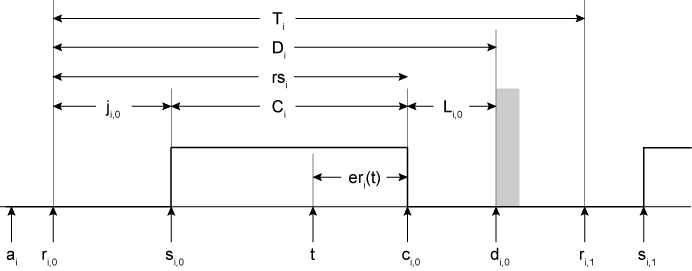
\includegraphics[width=0.7\textwidth]{master-exam-2014/figure1}
 
\item In the rate monotonic algorithm, the task with the ........... gets the highest static priority. ( Please fill in the blank )

\item In the earliest deadline algorithm, the task with the ............... gets the highest dynamic priority. ( Please fill in the blank )

\end{unteraufgaben}

\pagebreak

\aufgabe{}{10}


14.	The rate monotonic algorithm is a static priority scheduling algorithm and the earliest deadline first is a dynamic priority scheduling algorithm. Using T1 = ( 1, 4 ); T2 = ( 2, 6 ); T3 = ( 3, 8 ); where the value in parantheses are ( C, T ). Please assume the deadline to be the same as the period.

\begin{unteraufgaben}

\item	Calculate the processor utilization factor of the tasks for both the alorithms. Does the calculated factor suffice the schedulability test? Please answer why?
\item	Compute the hyperperiod of the tasks. 
\item	Fill in the chart to draw the schedulability of the tasks for both the algorithm.

\end{unteraufgaben}

\aufgabe{}{5}


Using T1 = ( 1, 4 ); T2 = ( 2, 8 ); T3 = ( 3, 12 ); where the value in parantheses are ( C, T ), please 

\begin{unteraufgaben}

\item	Calculate the processor utilization factor of the task using RM algorithm.
\item	Compute the hyperperiod of the task set. 
\item	Fill in the chart to draw the schedulability of the tasks using the RM algorithm.
\item	Can an aperiodic task with the release time of 2, deadline of 20 and computation time of 3 fit in this algorithm? Please calculate the response time of this aperiodic task.

\end{unteraufgaben}


\pagebreak

\aufgabe{}{5}

In the below precedence tasks with 9 tasks, please fill in the chart in accordance to the priority.

\begin{unteraufgaben}

\item	For a three processor system.
\item	For a four processor system. 

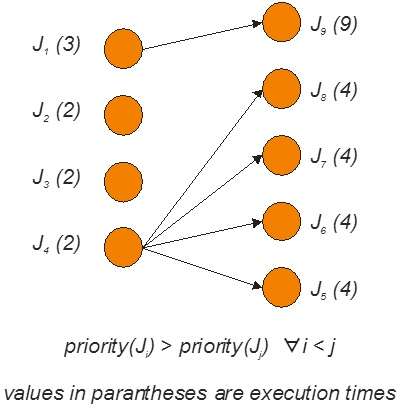
\includegraphics[width=0.5\textwidth]{master-exam-2014/figure2.jpg}

\end{unteraufgaben}




\end{document}

